

\section{Desirable Representations (RQ3)}
\label{sec:rq3}
To determine the overall trends in the data, we created and compared total orderings on the representations in each equivalence class (Figure~\ref{fig:refactoringTree})  with respect to the understandability (RQ1) and community standards (RQ2)   metrics.

\subsection{Analysis}
Total orderings were achieved by building directed graphs with the representations as nodes and edge directions determined by the metrics: matching and composition for understandability;  patterns and projects for community standards. Within each graph, a topological sort created total  orderings.

The graphs for understandability are based on Table~\ref{table:testedEdgesTable} and for community support are based on Table~\ref{table:nodeCount} and the graphs. 
%The following sections describe the process for building  and sorting the graphs. 



\subsubsection{Building the Graphs}
In the community standards graph, a directed edge  $\overrightarrow{C2  C1}$ is used when  nPatterns(C1) $>$ nPatterns(C2) \emph{and}  nProjects(C1) $>$ nProjects(C2).
When there is a conflict between nPatterns and nProjects, as is the case between L2 and L3, 
%where L2 is found in more patterns and L3 is found in more projects, 
an undirected edge $\overline{L2L3}$ is used. % as there is no winner based on the  metrics. 
The same process is used to identify directed and undirected edges based on community standards metrics. 
%After considering all pairs of nodes in each equivalence class that also have an edge in Figure~\ref{fig:refactoringTree}, we create graphs, 
For example, Figure~\ref{fig:graphsforanalysis} shows the graphs for  the CCC group; Figure~\ref{fig:graphsforanalysis}a is based on  understandability and Figure~\ref{fig:graphsforanalysis}b is based  on community standards. Nodes with fewer incoming edges are more smelly and nodes with more incoming edges are less smelly. 
%Note that with the CCC group, there is no edge between C3 and C5 because there is no straightforward refactoring between those representations, as discussed in Section~\ref{sec:refactoring}.

\begin{figure}[tb]
\centering
%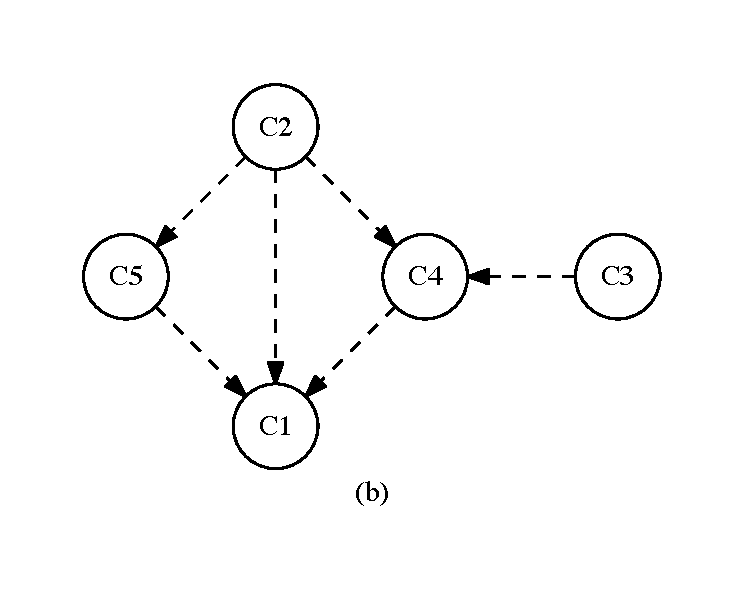
\includegraphics[width=0.57\columnwidth]{graphs/ccom.pdf}
%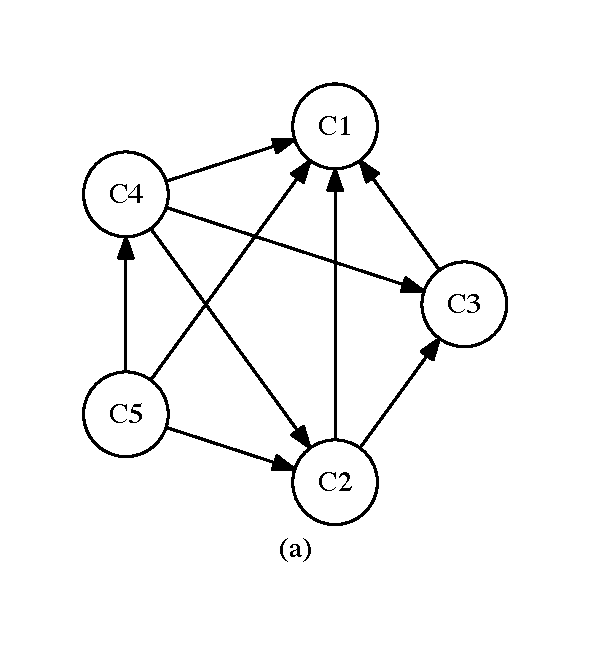
\includegraphics[width=0.40\columnwidth]{graphs/cart.pdf}
\includegraphics[width=0.57\columnwidth]{graphs/ccom.eps}
\includegraphics[width=0.40\columnwidth]{graphs/cart.eps}
\vspace{-12pt}
\caption{Trend graphs for the CCC equivalence graph: (a) represent the understandability analysis (RQ1) and (b) represent the artifact analysis (RQ2)}

\label{fig:graphsforanalysis}
\end{figure}


%\begin{table}
%\centering
%\caption{Topological Sorting, with the left-most position being highest \label{topologicalResults}}
%\begin{footnotesize}
%\begin{tabular}{| l | l | l | l | l | l |} \hline
%				& CCC			& DBB 		& LBW & SNG & LIT \\ \hline
%U 			& C1 C5 C4 C2 C3 	& D3 D1 D2 	& L3 L2		& S2 S1		& T1 T2 T4 T3 \\
%C		& C1 C3 C2 C4 C5 	& D2 D1 D3	&  L3 L2 L1 	& S2 S1 S3 	& T1 T3 T2 T4 \\
%\hline
%\end{tabular}
%\end{footnotesize}
%\end{table}

\begin{table}
\centering
\caption{Topological Sorting, with the left-most position being highest (non-smelly) and the right-most being most smelly \label{topologicalResults} \todo{make sure this matches new results}}
\vspace{-6pt}
\begin{tabular}{| l | l | l |}  \hline
& Understandability & Community  \\ \hline 
CCC & C1 C5 C4 C2 C3  &   C1 C3 C2 C4 C5  \\
DBB & D3 D1 D2  &   D2 D1 D3\\
 LBW & L3 L2	 &  L3 L2 L1 	\\
 SNG &  S2 S1 &  S2 S1 S3 \\
 LIT & T1 T2 T4 T3 & T1 T3 T2 T4 \\
\hline
\end{tabular}
\vspace{-6pt}
\vspace{-6pt}
\end{table}


%In the understandability graph, we represent a directed edge  $\overrightarrow{C2C1}$ when match(C1) $>$ match(C2) \emph{and} compose(C1) $>$ compose(C2). When there is a conflict between match and compose, as is the case with T1 and T3 where match(T1) is higher but compose(T3) is higher, an undirected edge $\overline{T1T3}$ is used. When one metric has a tie, as is the case with composition in E9, we use the other metric to determine  $\overrightarrow{C5C1}$. An example understandability graph for the CCC is shown in Figure~\ref{fig:graphsforanalysis}b. Nodes with few incoming edges are less understandable (or were not evaluated in our study), and nodes with more incoming edges were more understandable. 
%\footnote{When there are confounded representations, as is the case with E8, E4, and E5 which all use tranformations from the CCC and the LIT equivalence classes, we omit those from the understandability graph. This makes sense since all use a transformation between T1 and T4 strongly favoring T1. }

\subsubsection{Topological Sorting}
Once the graphs are built for each equivalence class and each set of metrics, we apply a modified version of Kahn's topological sorting algorithm to obtain a total ordering. 
%The first modification is to remove all undirected edges since Kahn's operates over a directed graph. 
%To begin, any disconnected nodes are added to the end of the topologically sorted list $L$. 
%In Kahn's algorithm, all nodes without incoming edges are added to a set $S$, which represents the order in which nodes are explored in the graph. For each $n$ node in $S$, all edges from $n$ are removed and $n$ is added to a list $L$. If there exists a node $m$ that has no incoming edges, it is added to $S$.  In the end, $L$ is a topologically sorted list.
%\begin{algorithm}
%  \caption{Modified Topological Sort}\label{topological}
%  \begin{algorithmic}[1]
%\State  $L \gets$ []
%\State $S \gets$ []
%\State Remove all undirected edges (creates a DAG) \label{removeundir}
%\State Add all disconnected nodes to $L$ and remove from graph. If there is more than one, mark the tie. \label{markTie1}
%\State Add all nodes with no incoming edges to $S$. If there is more than one, mark the tie. \label{addnoincomingtos}
%\While {$S$ is non-empty} \label{beginwhile}
%	\State remove a node $n$ from $S$ \label{setn}
%	\State add $n$ to $L$  \label{addntoL}
%	\For {node $m$ such that $e$ is an edge $\overrightarrow{nm}$}
%		\State remove $e$
%		\If{$m$ has no incoming edges}
%			\State add $m$ to $S$ \label{addToS}
%		\EndIf
%	\EndFor
%	\State If multiple nodes were added to $S$ in this iteration, mark the tie \label{markTie2}
%	\State remove $n$ from graph
%\EndWhile
%\State For all ties in $L$, use a tiebreaker.
%  \end{algorithmic}
%\end{algorithm}
One downside to Kahn's algorithm is that the total ordering is not unique and often multiple nodes with similar properties (e.g., no incoming edges) could be considered tied. Thus, we mark ties in order to identify when a tiebreaker is needed.
% to enforce a total ordering on the nodes (though admittedly, it is not always unique). 
%For example, on the understandability graph in Figure~\ref{fig:graphsforanalysis}, there is a tie between C3 and C2 since both have no incoming edges, so they are marked as a tie. Further, if C3 is added to $S$ first, when $n=C2$, both C5 and C4 are added to $S$, thus the tie between them is marked. In these cases, a tiebreaker is needed.
Breaking ties on the community standards graph involves choosing the representation that appears in a larger number of projects, as it is more widespread across the community. 
Breaking ties in the understandability graph uses the RQ1 results. Based on Table~\ref{table:testedEdgesTable}, we compute the average metrics for all instances of each representation. For example, C4 appears in E5, E12 and E13 with an overall average matching score of 0.81 and composition score of 24.3. C5 appears in E4 and E9 with an average matching of 0.87 and composition of 28.28. Thus, C5 is favored to C4 and appears higher in the sorting.

\subsection{Results}
The total orderings on nodes for each graph are shown in Table~\ref{topologicalResults}.  For example, given the graphs in Figure~\ref{fig:graphsforanalysis}a and Figure~\ref{fig:graphsforanalysis}b, the topological sorts are {\tt C1 C5 C4 C2 C3} and  {\tt C1 C3 C2 C4 C5}, respectively.



Considering both topological sorts, there is a clear winner in each equivalence class, with the exception of DBB.
%That is, the node sorted highest in the topological sorts for both the community standards and understandability analyses are 
This is C1 for CCC, L3 for LBW, S2 for SNG, and T1 for LIT.
Having a consistent and clear winner is evidence of a preference with respect to community standards and understandability, and thus provides guidance for potential refactorings.

%While the least-smelly representation is relatively clear, the smelliest representation varies.
%After the top rank, the second rank varies depending on the metric, however, h
This positive result, that the most popular representation in the corpus is also the most understandable, makes sense as people may be more likely to understand things that are familiar or well documented. However, while L3 is the winner for the LBW group, we note that L2 appears in slightly more patterns.
DBB is different  as the orderings are completely reversed depending on the analysis, so the community standards favor D2 and understandability favors D3. Further study is needed on this, as well as  LBW and SNG since not all nodes were considered in the understandability analysis. 
%

